\section{Experimental results}\label{header-n500}

\subsection{Metrics over the holdouts}\label{header-n501}

In this section the experimental results are reported. For each metric
(loss function value and accuracy) there are a table and a plot to
confront the learning machine performance. Each metric is calculated for
each model for each holdout and the final results are the mean and the
standard deviation of the metrics obtained over the holdouts. The values
are reported for both training and testing phases.

\newpage
\textbf{Accuracy}

\begin{longtable}[]{@{}lll@{}}
\toprule
\textbf{Models} & \textbf{Training} & \textbf{Test}\tabularnewline
\midrule
\endhead
Perceptron & mean = 0.9665 & mean = 0.9633\tabularnewline
& STD = 0.0016 & STD = 0.0035\tabularnewline
FFNN & mean = 0.9993 & mean = 0.9987\tabularnewline
& STD = 0.0008 & STD = 0.0009\tabularnewline
CNN\_1 & mean = 0.9982 & mean = 0.9969\tabularnewline
& STD = 0.0012 & STD = 0.0022\tabularnewline
CNN\_2 & mean = 0.9854 & mean = 0.9839\tabularnewline
& STD = 0.0074 & STD = 0.007\tabularnewline
CNN\_3 & mean = 0.8814 & mean = 0.8797\tabularnewline
& STD = 0.0239 & STD = 0.0252\tabularnewline
CNN\_4 & mean = 0.9627 & mean = 0.961\tabularnewline
& STD = 0.031 & STD = 0.0314\tabularnewline
\bottomrule
\caption{Accuracy and its standard deviation results for training and test sets}
\end{longtable}

\begin{figure}[h!]
	\centering
	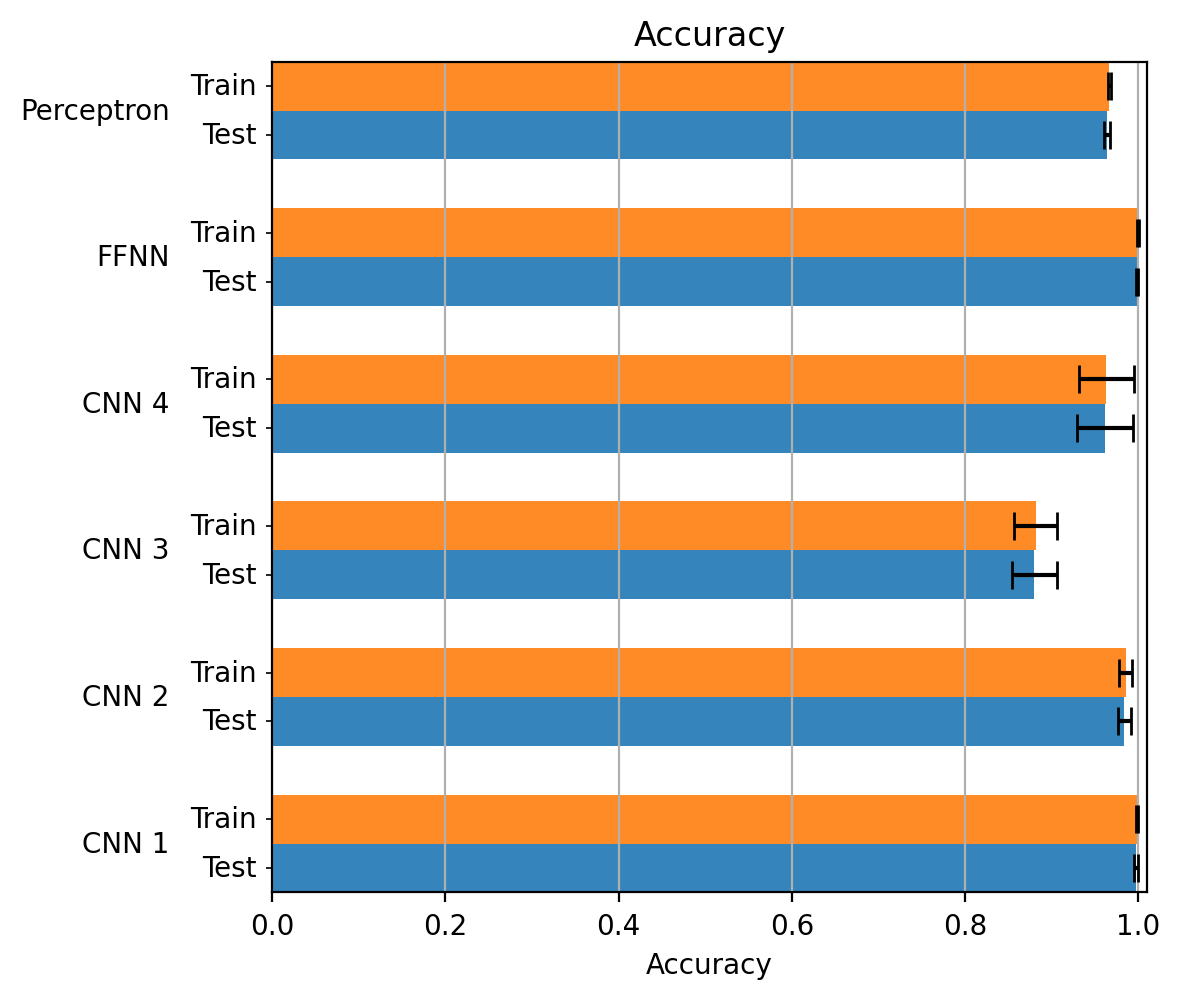
\includegraphics[width=0.85\linewidth]{../images/accuracy.png}
	\caption{Accuracy and its standard deviation results for training and test sets}
\end{figure}

\textbf{Loss function value}
\begin{longtable}[]{@{}lll@{}}
	\toprule
	\textbf{Models} & \textbf{Training} & \textbf{Test}\tabularnewline
	\midrule
	\endhead
	Perceptron & mean = 0.1529 & mean = 0.1584\tabularnewline
	& STD = 0.0043 & STD = 0.0069\tabularnewline
	FFNN & mean = 0.0095 & mean = 0.0109\tabularnewline
	& STD = 0.0051 & STD = 0.0053\tabularnewline
	CNN\_1 & mean = 0.0139 & mean = 0.0169\tabularnewline
	& STD = 0.005 & STD = 0.0071\tabularnewline
	CNN\_2 & mean = 0.0511 & mean = 0.0551\tabularnewline
	& STD = 0.0214 & STD = 0.0206\tabularnewline
	CNN\_3 & mean = 0.3454 & mean = 0.3487\tabularnewline
	& STD = 0.0659 & STD = 0.0664\tabularnewline
	CNN\_4 & mean = 0.1103 & mean = 0.117\tabularnewline
	& STD = 0.0885 & STD = 0.09\tabularnewline
	\bottomrule
	\caption{Loss function and its standard deviation results for training and test sets}
\end{longtable}



\begin{figure}[h!]
\centering
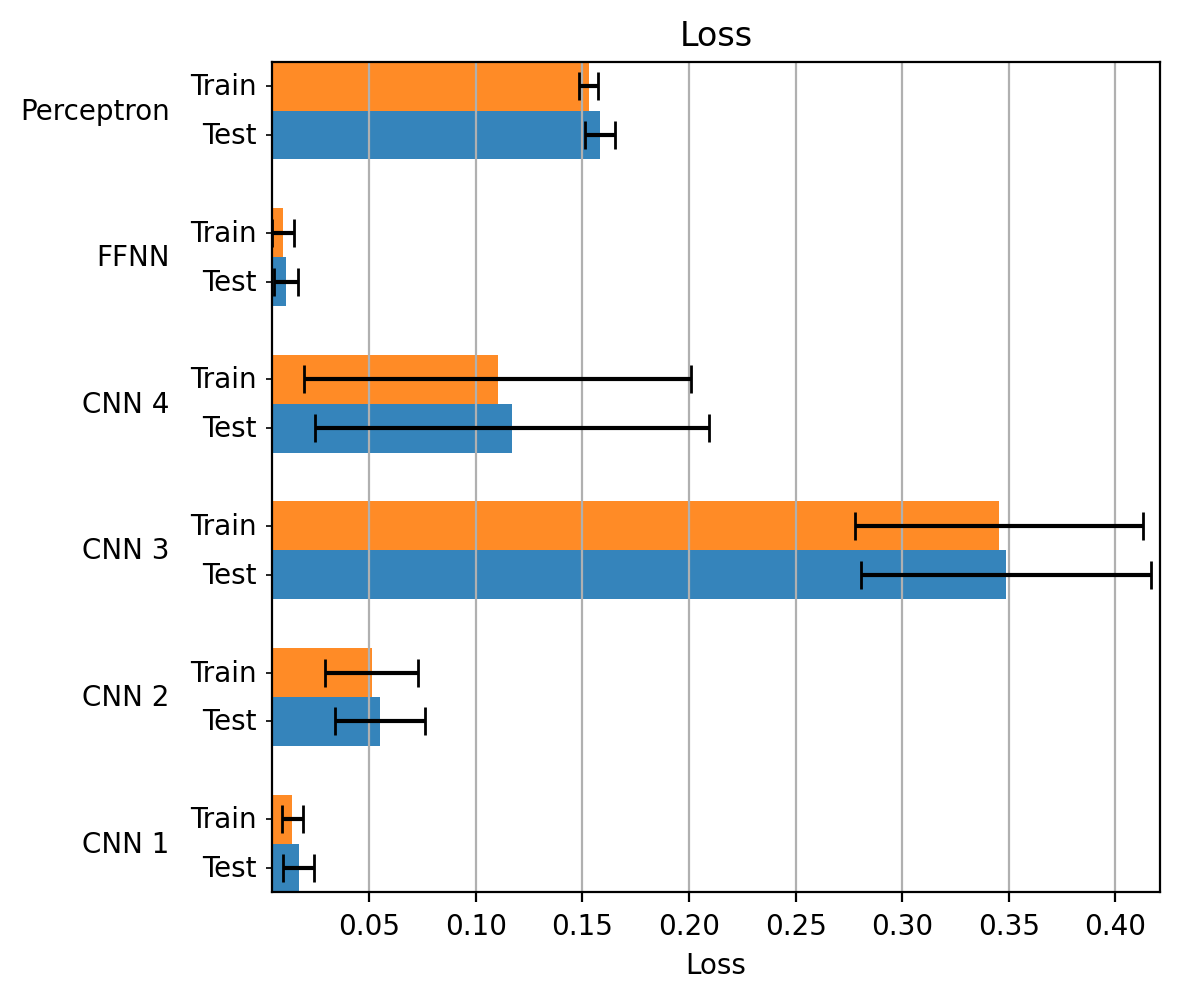
\includegraphics[width=0.85\linewidth]{../images/loss.png}
\caption{Loss function and its standard deviation results for training and test sets}
\end{figure}

\subsection{Metrics during training phase}\label{header-n613}

The following graphs show the trend of the metric for each model during
the training phase, calculated both on the training and test sets.

\textbf{Perceptron}

\begin{figure}[h!]
\centering
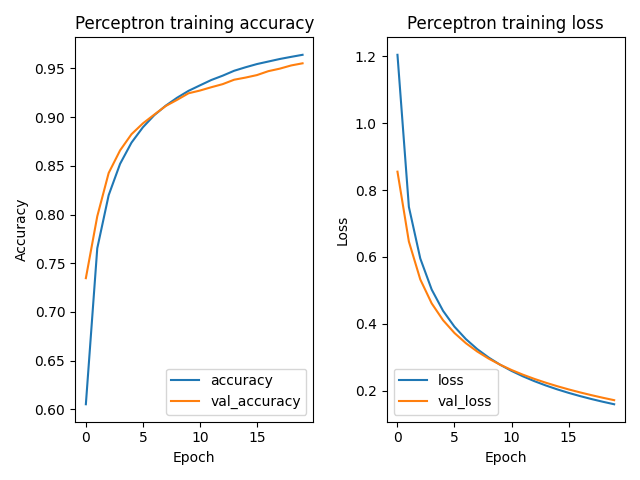
\includegraphics[width=0.68\linewidth]{../images/perceptron_training_accuracy.png}
\caption{\emph{Perceptron} accuracy and loss function value during training phase}
\end{figure}

\textbf{FFNN}

\begin{figure}[h!]
\centering
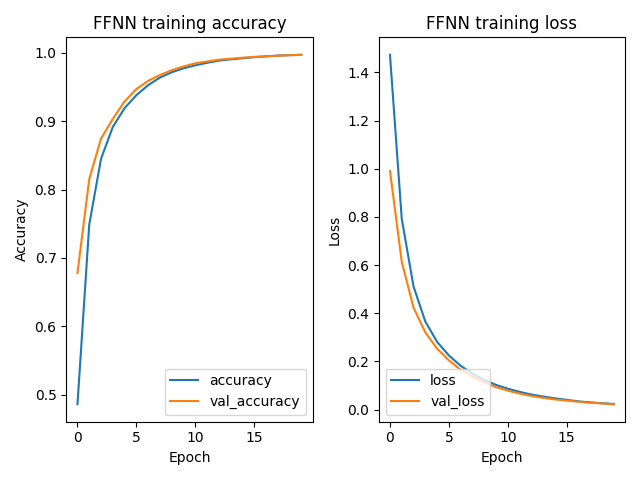
\includegraphics[width=0.68\linewidth]{../images/ffnn_training_accuracy.png}
\caption{\emph{FFNN} accuracy and loss function value during training phase}
\end{figure}

\textbf{CNN\_1}

\begin{figure}[h!]
\centering
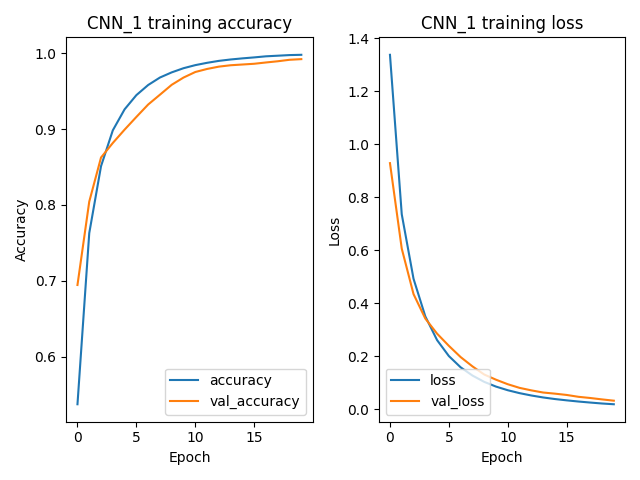
\includegraphics[width=0.68\linewidth]{../images/cnn_1_training_accuracy.png}
\caption{\emph{CNN\_1} accuracy and loss function value during training phase}
\end{figure}

\textbf{CNN\_2}

\begin{figure}[h!]
\centering
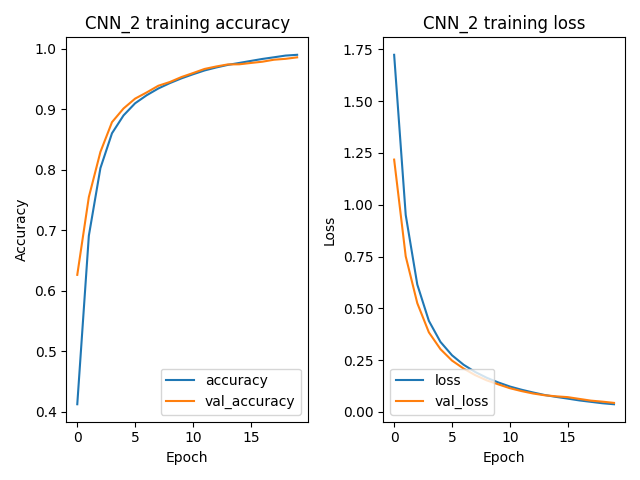
\includegraphics[width=0.68\linewidth]{../images/cnn_2_training_accuracy.png}
\caption{\emph{CNN\_2} accuracy and loss function value during training phase}
\end{figure}

\newpage

\textbf{CNN\_3}

\begin{figure}[h!]
\centering
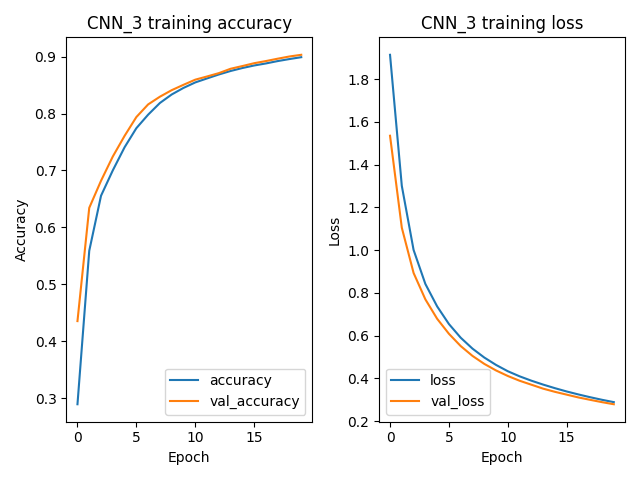
\includegraphics[width=0.68\linewidth]{../images/cnn_3_training_accuracy.png}
\caption{\emph{CNN\_3} accuracy and loss function value during training phase}
\end{figure}

\textbf{CNN\_4}

\begin{figure}[h!]
\centering
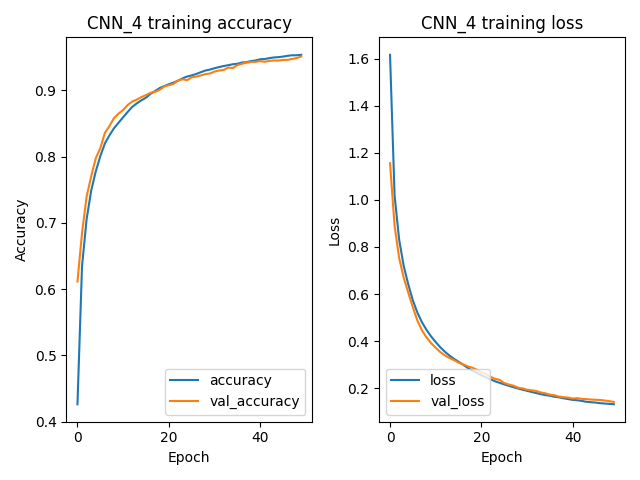
\includegraphics[width=0.68\linewidth]{../images/cnn_4_training_accuracy.png}
\caption{\emph{CNN\_4} accuracy and loss function value during training phase}
\end{figure}

\subsection{Observations}\label{header-n627}

The following observations are statistically validated using the
Wilcoxon test.

\emph{1) All neural networks used to execute the experiments performs
well.} The models get high accuracy results and low loss function
values. Their performances are great even if the training phase short:
the number of epochs is 20 for all models, with the exception of
\emph{CNN\_4} for which the number of epochs is 50. In particular, the
accuracy is always greater than 0.85, and the loss values smaller than
0.35.

\emph{2) Task simplicity requires simple models.} In general, the
models' performances degrade with an increase in complexity. The
simplest model (the \emph{Perceptron}) works better than the most
complicated one (\emph{CNN\_3}). The complexity of the latter requires a
longer training phase to increase its performance. The prove of this is
\emph{CNN\_4}, which has the same architecture as \emph{CNN\_3}, but the
number of epochs is higher and the batch size lower. In this way, the
model can learn more and faster. Despite this, the standard deviation
grows both for accuracy and loss function value: the network performance
strongly depends on the holdout used for training the network.

\emph{3) The overfitting problem does not exist.} No model produces
overfitting, even the most complex ones. This means that data is simply
to learn and all of them are characterize from common patterns.

\emph{4) FFNN is the best model.} The Wilcoxon test confirms that
\emph{FFNN} is the network with higher performance in the validation
phase, overcoming also \emph{CNN\_1}. Despite this is true both for
accuracy and loss function value, it is more visible in the loss
function graphic.

\emph{5) CNN\_3 is the worst model.} This network has lower performance,
both for the training and validation phase, because the reduced number
of epochs does not allow the complex architecture of the network to
learn enough.

\section{Conclusions}\label{header-n631}

The image multi-classification task described in this project is
relatively simple if it is addressed using deep learning models. The two
main reasons concern the dataset characteristics and the task's
simplicity. The dataset is composed of pictures that depict only the
fruit and vegetables to classify, without other objects that can add
noise. In this way, the models learn only the feature that characterizes
the target classes. In addition, the images represent the subject in
different positions and light conditions. This fact allows to avoid the
image augmentation technique during the pre-processing phase. Simple
models work better because of the task's simplicity. Compared to more
complex models, their performance is higher, they learn faster and the
standard deviation is lower. The best one is a simple feed-forward
neural network, which works better than all convolutional neural network
tested in the experiments.

\end{document}
